\documentclass[tikz,border=4pt]{standalone}
\usepackage{pgfplots}
\pgfplotsset{compat=1.16}
\pgfplotsset{
  bode/.style={
    width=6.4cm, height=4.4cm, xmin=1, xmax=10000,
    xtick={1,10,100,1000,10000},
    grid=both, major grid style={gray!55}, minor grid style={gray!20},
    tick label style={font=\footnotesize}, label style={font=\small},
    title style={font=\small}, xlabel={$f$ [Hz]},
  },
  bode mag/.style={bode, ymin=-60, ymax=10, ytick={-60,-40,-20,0},
    ylabel={$|G|_{\mathrm{dB}}$}, title={Modulo}},
  bode fase/.style={bode, ymin=-100, ymax=10, ytick={-90,-45,0},
    ylabel={$\varphi$ [$^\circ$]}, title={Fase}},
}
% R = 680 ohm, C = 4.7 uF  ->  fc = 1/(2 pi R C) = 49.798 Hz
\def\wc{49.798}
\begin{document}
% G(j w) = 1/(1 + j w R C)
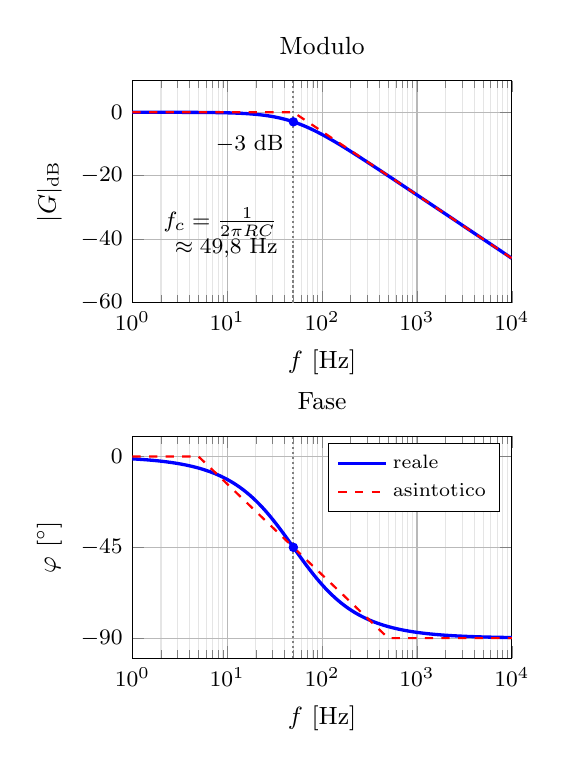
\begin{tikzpicture}
% ---------- modulo ----------
\begin{semilogxaxis}[bode mag, name=mag]
  \addplot[blue, very thick, domain=0:4, samples=121] ({10^x}, {-10*log10(1+(10^x/\wc)^2)});
  \addplot[red, thick, dashed] coordinates {(1,0) (\wc,0) (10000,-46.06)};
  \addplot[gray, thick, densely dotted, forget plot] coordinates {(\wc,-60) (\wc,10)};
  \addplot[only marks, mark=*, mark size=1.5pt, blue, forget plot] coordinates {(\wc,-3.01)};
  \node[anchor=north east, font=\footnotesize] at (axis cs:\wc,-4) {$-3$ dB};
  \node[anchor=east, font=\footnotesize, align=right]
    at (axis cs:43,-38) {$f_c=\frac{1}{2\pi RC}$\\$\approx 49{,}8$ Hz};
\end{semilogxaxis}

% ---------- fase ----------
\begin{semilogxaxis}[bode fase, at={(mag.south)}, yshift=-1.7cm, anchor=north,
  legend style={font=\scriptsize, at={(0.97,0.97)}, anchor=north east},
  legend cell align=left]
  \addplot[blue, very thick, domain=0:4, samples=121] ({10^x}, {-atan(10^x/\wc)});
  \addplot[red, thick, dashed] coordinates {(1,0) (4.9798,0) (497.98,-90) (10000,-90)};
  \legend{reale, asintotico}
  \addplot[gray, thick, densely dotted, forget plot] coordinates {(\wc,-100) (\wc,10)};
  \addplot[only marks, mark=*, mark size=1.5pt, blue, forget plot] coordinates {(\wc,-45)};
\end{semilogxaxis}
\end{tikzpicture}
\end{document}